\chapter{A Teoria da Medida}
%%%%%%%%% ESPAÇOS MENSURÁVEIS
    Nesta seção, apresentaremos o conceito chave deste trabalho: a teoria da medida.
    Para isso, precisaremos ampliar o conjunto dos números reais para que ele possa atender novas exigências.
    Isso é necessário porque, as vezes, teremos conjuntos tão \enquote{grandes} que nenhum número real poderá representar sua \enquote{medida}. 
    Assim, estenderemos o conjunto dos números reais na primeira seção.
    Na seguinte, estenderemos o conceito de função mensurável para o conjunto dos números reais estendidos e, na seção final, apresentaremos a definição de medida bem como exemplos dela.
    
\section{Os Espaços de Funções Mensuráveis}
	Adiante apresentaremos conjuntos tão \enquote{grandes} que nenhum número real poderá expressar seu \enquote{tamanho}.
	Assim, antes de prosseguirmos expandiremos o conjunto da reta real que temos trabalhado anteriormente.
    \begin{env}{Definição}
    \label{def:reta-estendida}
        O sistema estendido de números reais, denotado por $\xreta$, consiste do corpo
        \footnote{
        \enquote{Um \textit{corpo} é um conjunto $K$, munido de duas operações, chamadas \textit{adição} e \textit{multiplicação}, que satisfazem a certas condições,chamadas os \textit{axiomas de corpo}[...]}
        \cite[p.61]{elon}. Os axiomas que ele se refere são as propriedades comutativa, associativa, elemento neutro e elemento simétrico para ambas operações juntamente com  
        a propriedade distributiva.
    	} 
        dos números reais $\R$ e dos símbolos $+\infty$ e $-\infty$, isto é, $\R \cup \{-\infty, +\infty\}$.
        \index{Sistema estendido de números reais}
    \end{env}
	
	Assim, nós preservamos a ordem original de $\R$ e definimos
	$-\infty < x < +\infty$ para todo $x \in \R$.
	Fica então claro que $+\infty$ é uma cota superior
	\index{Cota superior}
	\footnote{
		\enquote{
		Um subconjunto $X$ de um corpo ordenado $K$ chama-se limitado superiormente quando existe $b \in K$ tal que 
		$b \geq x$ para todo $x \in X$. 
		Em outras palavras, tem-se $X \subset (-\infty, b]$.
		Cada $b \in K$ com esta propriedade chama-se uma cota superior de $X$
		} \cite[p.74]{elon}.
	} 
	de cada subconjunto do estendido sistema de números reais, e que todo subconjunto não vazio tem um supremo
	\index{Supremo}
	\footnote{
		\enquote{
		Sejam $K$ um corpo ordenado e $X \subset K$ um subconjunto limitado superiormente. 
		Um elemento $b \in K$ chama-se supremo do subconjunto $X$ quando $b$ é a menor das cotas superiores de $X$ em	$K$
		} \cite[p.75]{elon}.
	}.
	Se, por exemplo, $E$ é um conjunto não vazio de números reais que não é limitado superiormente em $\R$, então $\sup E = + \infty$ no sistema de números reais estendido
	\footnote{
	Exatamente as mesmas observações se aplicam aos limites inferiores.
	Essas definições podem ser encontradas em \cite[p.12]{rudin}.
	}.
	
    Com isso, parece que nosso problema de \enquote{medir} conjuntos muito grandes se resolveu.
    Entretanto, alguns cuidados são necessários para operarmos em $\xreta$.
    Note que $\xreta$ não é um corpo, pois não é fechado para operação de adição uma vez que $(+\infty) + (-\infty)$ não é definido.
    Dito isso, para $x \in \R$, aplicaremos as seguintes convenções:
    \begin{enumerate}[label*=(\alph*)]
    	\item Se $x > 0$, então $x \cdot (+\infty) = +\infty, x \cdot (-\infty) = -\infty$;
    	\item Se $x < 0$, então $x \cdot (+\infty) = -\infty, x \cdot (-\infty) = +\infty$;
    	\item Se $x = 0$, então 
    	$x\cdot (+\infty) = x\cdot (-\infty) = 0$;
    	\item $(+ \infty) + (+ \infty)  = x + \infty = (+ \infty) \cdot  (+ \infty) = (- \infty) \cdot (- \infty) = + \infty$;
    	\item $(- \infty) + (- \infty)  = x - \infty = (- \infty) \cdot  (+ \infty) = (+ \infty) \cdot (- \infty) = - \infty$.
    \end{enumerate}
    
    Neste novo contexto de números reais a \sigal de Borel não é mais válida uma vez que a \ref{def:algebra-borel} não inclui $+\infty$ nem $-\infty$.
    Logo, precisaremos de uma $\sigma$-álgebra em $\xreta$ para dar continuidade aos nossos estudos. 
    Com isso, considere $\xreta$.
    Tomando um conjunto arbitrário $E \in \borel$, com $\varnothing \neq E$, defina $E_1 = E \cup \{-\infty\}, E_2 = E \cup \{+\infty\}$ e $E_3 = E \cup \{-\infty, +\infty\}$. Com isso podemos fazer o seguinte enunciado: 
    % Desta forma, o conjunto $\overline{\borel} = \displaystyle \bigcup_{E \in \borel} \{E, E_1, E_2, E_3\}$ é uma \sigal de $\xreta$.
    \begin{comment}
    Com efeito, se $E \in \borel$, então é um intervalo aberto conforme o teorema \ref{teo:equiv-borel}.
    Assim, $E_1, E_2, E_3$ e $E_4$ serão intervalos do tipo $[-\infty,x)$ ou $(x, +\infty]$ que são elementos de $\borel$ acrescidos de $+\infty$ ou $-\infty$. 
    Deste modo, é fácil verificar que se um elemento $A \in \xborel$, então $A^c \in \xborel$.
    Além disso, a união enumerável é, no máximo, o intervalo $[-\infty,+\infty]$ que é exatamente $\xreta$.
    Desta forma, $\xborel$ é uma \sigal de $\xreta$.
    	
    \end{comment}
    
    \begin{env}{Definição}
    \label{def:algebra-borel-estendida}
        A \sigal $\overline{\borel} = \displaystyle \bigcup_{E \in \borel} \{E, E_1, E_2, E_3\}$ do conjunto $\xreta$ é chamada de $\sigma$-álgebra de Borel Estendida.
        \index{$\sigma$-álgebra! de Borel estendida}
    \end{env}

    Uma vez que estamos familiarizados com os conceitos de funções de valores reais mensuráveis, estamos prontos para estender este conceito para o conjunto $\xreta$.
    \begin{env}{Definição}
    \label{def:familia-funcoes-mensuraveis}
        Sendo $(X, \mathcal{C})$ um espaço mensurável, uma função de valores reais estendidos $f: X \to \xreta$ é dita $\mathcal{C}$-mensurável caso o conjunto
        $\{x \in X; f(x) > \alpha\} \in \mathcal{C}$ para qualquer que seja $\alpha \in \R$. 
        \vspace{-0.4cm}
    \end{env}

	Denotaremos a família de todas as funções de valores reais estendidos de $X$ que são $\mathcal{C}$-mensuráveis por $M(X, \mathcal{C})$.
	Além disso, caso estivermos tratando apenas das funções não negativas usaremos $M^+(X, \mathcal{C})$.
    \begin{env}{Proposição}
    \label{prop:identidade-intersecao-mais-infinito}
        Se $f \in \menfus$, então $\{x \in X; f(x) = +\infty\} = \displaystyle \bigcap_{n = 1}^\infty \{x \in X; f(x) > n\}$.
        Em particular, $\{x \in X; f(x) = +\infty\} \in \cc$.
    \end{env}
    \begin{prova}
        Tome, de modo arbitrário, um elemento $a \in X$. 
        Assim, 
        \begin{align*}
            a \in \bigcap_{n = 1}^\infty \{x \in X; f(x) > n\} 
            \Leftrightarrow &\ a \in \{x \in X; f(x) > n\}, \ \forall\  n \in \N\\
            \Leftrightarrow &\  \forall\ n \in \N,\ f(a) > n\\
            \Leftrightarrow & f(a) = +\infty.  
        \end{align*}
    Além disso, note que cada $\{x \in X;\, f(x) > n\} \in \mathcal{C}$.
    Segue, pela \ref{prop:interseção-elementos-sigmas}, que \linebreak $\displaystyle \bigcap_{n = 1}^\infty \{x \in X; f(x) > n\} \in \mathcal{C}$ acarretando que $\{x \in X; f(x) = +\infty\} \in \mathcal{C}$. 
    \end{prova}

    \begin{env}{Proposição}
    \label{prop:identidade-união-menos-infinito}
        Se $f \in \menfus$, então $\{x \in X; f(x) = -\infty\} = \displaystyle \left(\bigcup_{n = 1}^\infty \{x \in X; f(x) > - n\}\right)^c$.
        Particularmente, $\{x \in X; f(x) = -\infty\} \in \cc$.
        \vspace{-0.4cm}
    \end{env}
	%
    \begin{prova}
    	Por hipótese, $f \in \menfus$.
    	Assim, pela \ref{prop:aritmetica-uma-funcao}, 
    	$-f \in \menfus$.
    	Logo, pela \ref{prop:identidade-intersecao-mais-infinito}, temos que 
    	$\{x \in X; -f(x) = +\infty\} = \displaystyle \bigcap_{n = 1}^\infty \{x \in X; -f(x) > n\}$.
    	Note que 
        \begin{align*}
            \bigcap_{n = 1}^\infty \{x \in X; -f(x) > n\}
            =& \bigcap_{n = 1}^\infty \{x \in X; f(x) < -n\}\\
            =& \bigcap_{n = 1}^\infty \{x \in X; f(x) \geq -n\}^c\\
            =& \left(\bigcup_{n = 1}^\infty \{x \in X; f(x) \geq -n\}\right)^c 
        \end{align*}
    	e que $\{x \in X; -f(x) = +\infty\} = \{x \in X; f(x) = -\infty\}$. Portanto, 
    	$$
    	\{x \in X; f(x) = -\infty\} 
    	= 
    	\displaystyle \left(\bigcup_{n = 1}^\infty \{x \in X; f(x) \geq -n\}\right)^c.$$
    \end{prova}
    \begin{env}{Teorema}
    \label{teo:condição-de-mensurabilidade}
        Uma função de valores reais estendidos $f: X \to \xreta$ é $\cc$-mensurável se, e somente se, os conjuntos 
        $A = \{ x \in X; f(x) = +\infty\}$ e $B = \{x \in X; f(x) = -\infty\}$
		 são elementos de $\mathcal{C}$ e a função $h: X \to \R$ definida por
		 \vspace{-0.2cm}
		 $$
		 h(x) = \left\{\begin{array}{cc}
		     f(x), & \textrm{\ se } x \notin A\cup B  \\
		      0,& \textrm{\ se } x \in A\cup B
		 \end{array}\right.
	 	 \vspace{-0.2cm}
		 $$
		 é $\cc$-mensurável.
		 \vspace{-0.2cm}
	 \end{env}
\begin{prova}
    Suponha que $f \in \menfus$. 
    Logo, pela \ref{prop:identidade-intersecao-mais-infinito} e \ref{prop:identidade-união-menos-infinito}, os conjuntos $A$ e $B$ são elementos de $\mathcal{C}$.
    Assim, tome $\alpha \in \R$ com $\alpha \geq 0$, então os elementos de $\{x \in X; h(x) > \alpha\}$ são os elementos de $\{x \in X; f(x) > \alpha\}$ que não estão em $A$, pois $h$ tem contradomínio $\R$.
    Como $\cc$ é uma \sigal\hspace{-0.1cm}, $A \in \cc \Rightarrow A^c \in \cc$. 
    Com isso, 
    \vspace{-0.2cm}
    $$
    \{x \in X; h(x) > \alpha\} = A^c\cap \{x \in X; f(x) > \alpha\} \in \cc.
    \vspace{-0.2cm}
    $$
    Segue, pela  \ref{prop:interseção-elementos-sigmas} que $\{x \in X; h(x) > \alpha\} \in \cc$, ou seja, $h$ é $\cc$-mensurável.
    Caso, $\alpha < 0$, então $\{x \in X; h(x) > \alpha\} = \{x \in  X ; f(x) > \alpha\} \cup B $, pois $h(x) = 0$ para $x \in A \cup B$.
    Desta forma $h$ é $\cc$-mensurável.

    Por outro lado, se supormos que $A$ e $B$ são elementos de $\mathcal{C}$ e $h$ é $\cc$-mensurável, então
    $
    \{x \in X; f(x) > \alpha\} 
    = 
    \{x \in  X ; h(x) > \alpha\} \cup A
    $
    quando $\alpha \geq 0$, e 
    $
    \{x \in X; f(x) > \alpha\} 
    = 
    \{x \in  X ; h(x) > \alpha\} \cap B^c 
    $
    quando  $\alpha < 0$, por motivos análogos à primeira parte da demonstração.
    Portanto, $f$ é uma função $\cc$-mensurável como desejávamos.
\end{prova}

Como consequência do \ref{prop:aritmetica-uma-funcao} e o \ref{teo:condição-de-mensurabilidade} obtemos, imediatamente, que se $ f \in M(X,\mathcal{C})$, então as funções $cf, f^2, |f|, f^+$ e $f^-$ também são elementos de $M(X, \mathcal{C})$.
Entretanto, um resultado análogo à \ref{prop:aritmetica-duas-funcoes} não é possível em $\xreta$.
Isso acontece porque em $\xreta$ a operação de adição não é bem definida.
Então caso $f(x) = +\infty$ e $g(x) = -\infty$ para algum $x \in \R$ a adição
$f(x) + g(x)$ não é realizada.
Por outro lado, a função $fg$ é $\cc$-mensurável se $f$ e $g$ forem ambas $\cc$-mensuráveis.
Antes disso, lembraremos de dois conceitos importantes nos estudos de análise: limite superior e inferior.

Seja $(x_n)$ uma sequência limitada de números reais.
Então existem $\alpha, \beta \in \R$ tais que $\alpha \leq x_n \leq \beta$ para todo $n \in \N$.
Denotando $X_n =\{x_n, x_{n+1}, ...\}$ podemos perceber que 
$X_n \subset [\alpha, \beta]$ para cada $n$ e que $X_1 \supset X_2 \ldots X_n \supset \ldots$
Definimos o limite superior e inferior pondo, respectivamente, 
\begin{center}
	$\displaystyle
	\lim_{n \to \infty}\sup X_n 
	=\sup_{n \to \infty} \left\{\inf X_n\right\}
	$
	e
	$\displaystyle
	\lim_{n \to \infty}\inf X_n 
	=\inf_{n \to \infty} \left\{\sup X_n\right\}
	$
\end{center}
\index{Limite! superior}
\index{Limite! inferior}
Podemos relacionar esses conceitos com as funções mensuráveis conforme o teorema a seguir:
\begin{env}{Teorema}
\label{teo:mensurabilidade-sequencia-funcoes-mensuraveis}
	Seja $(f_n)$ uma sequência de elementos de $\menfus$ e defina as funções
	$\displaystyle
	f(x) = \inf_{n \to \infty} f_n(x),\  
	F(x) = \sup_{n \to \infty} f_n(x),\  
	f^*(x) = \lim_{n \to \infty}\inf f_n(x)$ e
	$\displaystyle 
	F^*(x) = \lim_{n \to \infty}\sup f_n(x).$
	Então as funções $f, f^*, F$ e $F^*$ são elementos de $\menfus$.
\end{env}
\begin{prova}
	Como $(f_n)$ é uma sequência de funções $\cc$-mensuráveis e 
	$\displaystyle f = \inf_{n \to \infty} f_n$, afirmamos que $\{x \in X; f(x) \geq \alpha\} = \displaystyle \bigcap_{n = 1}^\infty \{x \in X; f_n(x) \geq \alpha\}$.
	De fato, tomemos um elemento $y \in X$.
	Assim, 
		\begin{align*}
			y \in \bigcap_{n = 1}^\infty \{x \in X; f_n(x) \geq \alpha\} 
			\Leftrightarrow&
			y \in \{x \in X; f_n(x) \geq \alpha\}\ \forall\  n \in \N\\
			\Leftrightarrow&	
			f_n(y) \geq \alpha\ \forall \ n \in \N \\
			\Leftrightarrow	&	
			\inf_{n \to \infty}f_n(y) \geq \inf_{n \to \infty}\alpha\ \forall \ n \in \N\\
			\Leftrightarrow	&	
			f(y) \geq \alpha\ \forall\  n \in \N\\
			\Leftrightarrow	&
			y \in \{x \in X; f(x) \geq \alpha\}
		\end{align*}
	Como cada $\{x \in X; f_n(x) \geq \alpha\}$ é $\cc$-mensurável, segue pela \ref{prop:interseção-elementos-sigmas} que o conjunto $\{x \in X; f(x) \geq \alpha\} \in \cc$ para todo $\alpha \in \R$.
	Desta forma, $f$ é $\cc$-mensurável.
	
	Além disso, por hipótese $(f_n)$ é uma sequência de funções mensuráveis.
	Logo, pela \ref{prop:aritmetica-uma-funcao}, a sequência $(-f_n)$ também é composta de funções mensuráveis.
	Logo, da primeira parte dessa demonstração, a função 
	$ g = -\inf (-f_n)$ é mensurável.
	lembre que, por propriedades de supremo e ínfimo
	\footnote{
		Especificamente o exercício 35 encontrado em \cite[p.92]{elon}.
		}, 
	$F = \sup f_n = -\inf(-f_n)$. 
	Disso, $F$ também é uma função $\cc$-mensurável.
	
	Note que a mensurabilidade de $f^*$ e $F^*$ vem da mensurabilidade de $f$ e $F$ uma vez que
	$$
	f^*(x) = \sup_{n \geq 1} \left\{\inf_{m \geq n} f_m(x)\right\}
	\textrm{\ e\ }
	F^*(x) = \inf_{n \geq 1} \left\{\sup_{m \geq n} f_m(x)\right\}
	$$
\end{prova}
\begin{env}{Corolário}
	\label{cor:convergencia-de-uma-sequencia-mensuravel}
	Se $(f_n)$ é uma sequência em $\menfus$ que converge
	\footnote{
		A convergência que nos referimos é a convergência pontual.
	} para $f$ em $X$, então
	$f$ também está em $\menfus$.
\end{env}
\begin{prova}
	Ora, por hipótese $\displaystyle f(x) = \lim_{n \to \infty} f_n(x)$.
	Só que $\displaystyle \lim_{n \to \infty} f_n(x) = \lim_{n \to \infty} \inf f_n(x)$.
	Segue que $\displaystyle f(x) = \lim_{n \to \infty} \inf f_n(x)$ que, por sua vez, é $\cc$-mensurável pelo teorema anterior.
\end{prova}

Para mostrar que o produto de duas funções mensuráveis em $\xreta$ é mensurável, precisamos ainda de um tipo particular de função que é definida adiante:
% Parte final do Capítulo - Truncamento
\begin{env}{Definição}
	Seja $f$ uma função em $\menfus$ e $A > 0$.
	Definimos o truncamento $f_A$ da função $f$ por
	$$ f_A(x) =
	\left\{\begin{array}{cc}
		f(x), & \textrm{se\ } |f(x)| \leq A \\
		A, & \textrm{se\ } f(x) > A \\
		-A, & \textrm{se\ } f(x) < -A.
	\end{array}\right.
	\vspace{-0.4cm}
	$$
	\index{Truncamento de uma função}
\end{env}
\begin{env}{Proposição}
	\label{prop:truncamento-mensurável}
	Seja $A$ um número real maior que zero.
	Se $f$ é uma função em $\menfus$, então $f_A$ é uma função $\cc$-mensurável.
\end{env}
\begin{prova}
	Basta provar que para qualquer que seja $\alpha \in \R$, tem-se $\{x \in X; f_A(x) > \alpha\} \in \cc$.
	Para isso, vamos analisar os casos de $\alpha$.
		\begin{enumerate}[label*=(\Roman*)]
			\item $\alpha = A$. 
			Assim, 
			$
			\{x \in X; f_A(x) > \alpha\}
			=
			\{x \in X; f_A(x) > A\}
			= \varnothing
			$, pois a função $f_A$ não assume valor maior que $A$.
			%
			\item $-A \leq \alpha < A$.
			Esse caso gera dois novos casos à analisar:
				\begin{enumerate}
					\item $\alpha < f(x) < A$. 
					Disso, 
					$
					-A \leq \alpha < f(x) < A
					\Rightarrow
					|f(x)| < A
					$.
					Logo, $f_A = f$, ou seja, $f_A$ é mensurável.
					\item $f(x) > A$.
					Logo, por definição, $f_A(x) = A$, isto é, $f_A$ é constante.
					Segue do \ref{ex:funcao-constante} que $f_A$ é mensurável.
				\end{enumerate} 
			$
			\{x \in X; f_A(x) > \alpha\}
			=
			\{x \in X; f(x) > \alpha\}
			\in \cc
			$, 
			pois $f$ é mensurável.
			%
			\item $\alpha < -A$.
			Ocorre que
			$
			\{x \in X; f_A(x) > \alpha \} = X \in \cc.
			$
			Pois todos os valores que $f_A$ assume são maiores ou igual à $-A$.
		\end{enumerate}
	Em todo caso, o conjunto $\{x \in X; f_A(x) > \alpha\}$ é um elemento de $\cc$.
	Portanto, $f_A$ é $\cc$-mensurável. 
\end{prova}
% Exemplo de Truncamento

Para que possamos entender melhor o truncamento de uma função, vamos observar o gráfico da função $g(x) = 3\cos(2x)$ apresentada na figura
\ref{fig:3cosseno_de_2x}. 
	\begin{figure}[h!]
		\centering
		\Caption{\label{fig:3cosseno_de_2x} Gráfico da função $g(x) = 3\cos (2x)$} 
		\UECEfig{}{
			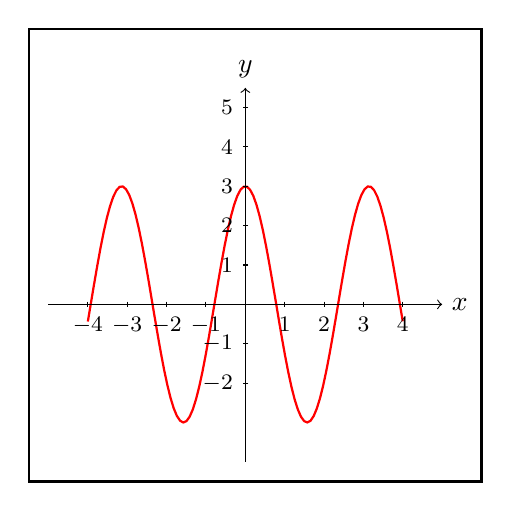
\begin{tikzpicture}[scale=0.5]
				\draw[thick] (-5.5, -4.5) rectangle (6, 7);
				% Defina o intervalo x
				\def\xmin{-3}
				\def\xmax{3}
				%				
				%				% Desenhe a função f(x)
				%				\draw[domain=\xmin+0.4:\xmax-0.4, smooth, samples=100, blue] plot (\x, {\x*\x -2});
				
				% Desenhando a função f_2
				\draw[domain=-4:4, thick, samples=100, red] plot (\x, {3*cos(2*\x r)});
				% Adicione rótulos aos eixos
				\draw[->] (\xmin-2,0) -- (\xmax+2,0) node[right] {$x$};
				\draw[->] (0,\xmin-1) -- (0,\xmax+2.5) node[above] {$y$};
				
				% Rótulos
				\foreach \i in {-4,-3,-2,-1,1,2,3,4}{
					\draw (\i,2pt)--(\i, -2pt) node[below]{{\footnotesize $\i$}};
				}
				
				\foreach \i in {-2, -1, 1,2,3,4,5}{
					\draw (2pt,\i)--(-2pt, \i) node[left]{{\footnotesize $\i$}};
				}
			\end{tikzpicture}
		}{
			\Fonte{Elaborado pelo autor}		}   
	\end{figure}
	Um truncamento faz, didaticamente falando, uma espécie de limitação no gráfico da função original.
	Ao tomarmos como constante o número real 1, vemos que o truncamento $g_1$ da função $g$, apresentada anteriormente, \enquote{amassa} o gráfico de $g$ nas ordenadas 1 e $-1$ como exposto na figura \ref{fig:truncamentog_1}.
		\begin{figure}[h!]
			\centering
			\Caption{\label{fig:truncamentog_1} Gráfico do truncamento $g_1$ } 
			\UECEfig{}{
				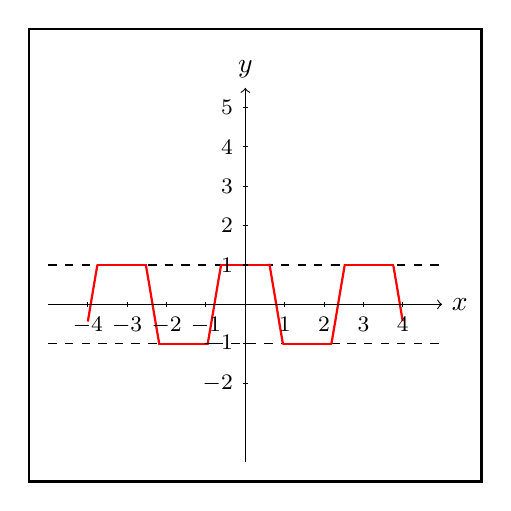
\begin{tikzpicture}[scale=0.5]
					\draw[thick] (-5.5, -4.5) rectangle (6, 7);
					% Defina o intervalo x
					\def\xmin{-3}
					\def\xmax{3}
					%				
					%				% Desenhe a função f(x)
					%				\draw[domain=\xmin+0.4:\xmax-0.4, smooth, samples=100, blue] plot (\x, {\x*\x -2});
					
					% Desenhando a função f_2
					%\draw[domain=-4:4, thick, samples=100, red] plot (\x, {3*cos(2*\x r)});
					\draw[domain=-5:5, dashed, samples=100] plot (\x, {1});
					\draw[domain=-5:5, dashed, samples=100] plot (\x, {-1});
					
					\draw[domain=-4:-3.755, thick, samples=100, red] plot (\x, {3*cos(2*\x r)});
					\draw[domain=-3.76:-2.55, thick, samples=100, red] plot (\x, {1});
					\draw[domain=-2.53:-2.18, thick, samples=100, red] plot (\x, {3*cos(2*\x r)});
					\draw[domain=-2.19:-0.96, thick, samples=100, red] plot (\x, {-1});
					\draw[domain=-0.96:-0.61, thick, samples=100, red] plot (\x, {3*cos(2*\x r)});
					\draw[domain=-0.61:0.635, thick, samples=100, red] plot (\x, {1});
					\draw[domain=0.61:0.96, thick, samples=100, red] plot (\x, {3*cos(2*\x r)});
					\draw[domain=0.96:2.19, thick, samples=100, red] plot (\x, {-1});
					\draw[domain=2.185:2.53, thick, samples=100, red] plot (\x, {3*cos(2*\x r)});
					\draw[domain=2.53:3.76, thick, samples=100, red] plot (\x, {1});]
					\draw[domain=3.76:4, thick, samples=100, red] plot (\x, {3*cos(2*\x r)});
					% Adicione rótulos aos eixos
					\draw[->] (\xmin-2,0) -- (\xmax+2,0) node[right] {$x$};
					\draw[->] (0,\xmin-1) -- (0,\xmax+2.5) node[above] {$y$};
					
					% Rótulos
					\foreach \i in {-4,-3,-2,-1,1,2,3,4}{
						\draw (\i,2pt)--(\i, -2pt) node[below]{{\footnotesize $\i$}};
					}
					
					\foreach \i in {-2, -1, 1,2,3,4,5}{
						\draw (2pt,\i)--(-2pt, \i) node[left]{{\footnotesize $\i$}};
					}
				\end{tikzpicture}
			}{
				\Fonte{Elaborado pelo autor}		}   
		\end{figure}	
	
Note que o mesmo ocorre com o truncamento $g_2$ apresentado na figura \ref{fig:truncamentog_2} onde, desta vez, $g$ é limitada pelas ordenadas $2$ e $-2$.
		\begin{figure}[h!]
			\centering
			\Caption{\label{fig:truncamentog_2} Gráfico do truncamento $g_2$ } 
			\UECEfig{}{
				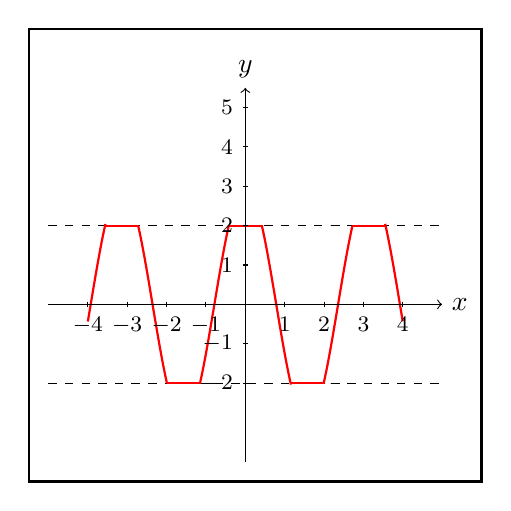
\begin{tikzpicture}[scale=0.5]
					\draw[thick] (-5.5, -4.5) rectangle (6, 7);
					% Defina o intervalo x
					\def\xmin{-3}
					\def\xmax{3}
					%				
					%				% Desenhe a função f(x)
					%				\draw[domain=\xmin+0.4:\xmax-0.4, smooth, samples=100, blue] plot (\x, {\x*\x -2});
					
					% Desenhando a função f_2
					%\draw[domain=-4:4, thick, samples=100, red] plot (\x, {3*cos(2*\x r)});
					\draw[domain=-5:5, dashed, samples=100] plot (\x, {2});
					\draw[domain=-5:5, dashed, samples=100] plot (\x, {-2});
					
					\draw[domain=-4:-3.552, thick, samples=100, red] plot (\x, {3*cos(2*\x r)});
					\draw[domain=-3.55:-2.71, thick, samples=100, red] plot (\x, {2});
					\draw[domain=-2.72:-1.99, thick, samples=100, red] plot (\x, {3*cos(2*\x r)});
					\draw[domain=-2:-1.15, thick, samples=100, red] plot (\x, {-2});
					\draw[domain=-1.15:-0.42, thick, samples=100, red] plot (\x, {3*cos(2*\x r)});
					\draw[domain=-0.43:0.43, thick, samples=100, red] plot (\x, {2});
					\draw[domain=0.42:1.16, thick, samples=100, red] plot (\x, {3*cos(2*\x r)});
					\draw[domain=1.15:2, thick, samples=100, red] plot (\x, {-2});
					\draw[domain=1.99:2.72, thick, samples=100, red] plot (\x, {3*cos(2*\x r)});
					\draw[domain=2.72:3.55, thick, samples=100, red] plot (\x, {2});]
					\draw[domain=3.552:4, thick, samples=100, red] plot (\x, {3*cos(2*\x r)});
					% Adicione rótulos aos eixos
					\draw[->] (\xmin-2,0) -- (\xmax+2,0) node[right] {$x$};
					\draw[->] (0,\xmin-1) -- (0,\xmax+2.5) node[above] {$y$};
					
					% Rótulos
					\foreach \i in {-4,-3,-2,-1,1,2,3,4}{
						\draw (\i,2pt)--(\i, -2pt) node[below]{{\footnotesize $\i$}};
					}
					
					\foreach \i in {-2, -1, 1,2,3,4,5}{
						\draw (2pt,\i)--(-2pt, \i) node[left]{{\footnotesize $\i$}};
					}
				\end{tikzpicture}
			}{
				\Fonte{Elaborado pelo autor}		}   
		\end{figure}
Assim, quanto maior o número $n$ do truncamento $g_n$ de uma função mensurável $g$, mais próximo o truncamento $g_n$ está de $g$ uma vez que a \enquote{limitação} vai desaparecendo.

Com esses resultados e observações podemos voltar a analisar o produto de duas funções com valores reais estendidos.
Considere $f,g \in \menfus$. 
Tomemos duas sequências $(f_k)$ e $(g_p)$ tais que para cada $k,p \in \N$, $f_k$ e $g_p$ são truncamentos de $f$ e $g$, respectivamente.
Ou seja,\vspace{0.5cm}
	\begin{minipage}{0.5\linewidth}
	$$ g_p(x) =
	\left\{\begin{array}{cc}
		g(x), & \textrm{se\ } |g(x)| \leq k \\
		p, & \textrm{se\ } g(x) > p \\
		-p, & \textrm{se\ } g(x) < p 
	\end{array}\right.	
	$$	
	\end{minipage}
e
	\begin{minipage}{0.5\linewidth}
		$$ f_k(x) =
		\left\{\begin{array}{cc}
			f(x), & \textrm{se\ } |f(x)| \leq k \\
			k, & \textrm{se\ } f(x) > k \\
			-k, & \textrm{se\ } f(x) < k 
		\end{array}\right.	
		$$	
	\end{minipage}
\vspace{0.5cm}

Pela \ref{prop:truncamento-mensurável}, $f_k$ e $g_p$ são $\cc$-mensuráveis para cada $k$ e $p$ números naturais.
Assim, pela \ref{prop:aritmetica-duas-funcoes}, $f_kg_p$ também é $\cc$-mensurável para quaisquer $k, p \in \N$.
Como mencionado anteriormente, o truncamento de uma função $f$ causa uma \enquote{limitação} em sua imagem.
Logo, se tomarmos $k$ grande o suficiente, o truncamento $f_k$ da função $f$ tende a se aproximar da própria função $f$.
Desta forma, fixemos um $p_0 \in \N$.
Assim, para $x \in X$
$$
\lim_{k \to +\infty} \left(f_k(x)g_{p_0}(x)\right) = f(x)g_{p_0}(x) 
$$
Segue pelo \ref{cor:convergencia-de-uma-sequencia-mensuravel} que 
$fg_{p_0} \in \menfus$. 
Analogamente, para $x \in X$
$$
\lim_{p \to +\infty} \left(f(x)g_p(x)\right) 
=
f(x)\cdot\lim_{p \to +\infty} g_p(x) 
= f(x)g(x) = (fg)(x)
$$
Concluímos, pelo mesmo corolário, que $fg \in \menfus$.
Com toda essa discussão, provamos as proposições:

\begin{env}{Proposição}
	\label{prop:convergencia do truncamento}
	Seja $f \in \menfus$ e $f_n$ um truncamento de $f$ para cada $n \in \N$. 
	Assim, para cada $x \in X, f_n(x)$ converge para $f(x)$ quando $n$ tende para $+\infty$.
\end{env}
\begin{env}{Proposição}
	\label{prop:produto de funções reais mensuraveis estendidas}
	Se $f$ e $g$ são duas funções mensuráveis de valores reais estendidos, então o produto $f \cdot g$ também é uma função mensurável de valor real estendido.
\end{env}

Dito isso, encerraremos esta subseção apresentando a definição generalizada de mensurabilidade de uma função.

\begin{env}{Definição}
	\label{def:mensurabilidade-geral}
	Sejam $(X, \cc)$ e $(Y,\mathcal{F})$ espaços mensuráveis.
	Dizemos que uma função $\varphi:X \to Y$ é mensurável se o conjunto $f^{-1}(E) = \{x \in X; f(x)\in E\} \in \cc$ para todo conjunto $E \in \mathcal{F}$. 
\end{env}
Embora essa definição pareça ser totalmente distinta da \ref{def:mensurabilidade-funções-reais}, as duas são equivalentes no caso particular de $Y = \R$ e $\mathcal{F} = \borel$ conforme demonstrado a seguir.

\begin{env}{Proposição}
	Seja $(X, \cc)$ um espaço mensurável e $f$ uma função.
	Então $f$ é $\cc$-mensurável se, e somente se, $f^{-1}(E) \in \cc$ para todo boreliano $E$. 
\end{env}
\begin{prova}
	Suponha $f$ uma função $\cc$-mensurável. 
	Sabemos pela \ref{def:algebra-borel} que os elementos da álgebra de Borel são gerados por intervalos do tipo $(-\infty,x)$ com $x \in \R$.
	Assim, dado arbitrariamente $\alpha \in \R$ temos que
	$$
	f^{-1}(-\infty, \alpha)
	=\{x \in X; f(x) \in (-\infty, \alpha)\}
	=\{x \in X; f(x) < \alpha\}
	\footnote{Por abuso de notação, $f^{-1}(-\infty, \alpha)$ \textrm{\ indica a pré imagem de\ } $(-\infty, \alpha)$.}.
	$$
	Como $f$ é $\cc$-mensurável segue pelo \ref{teo:equiv-funcoes-mensuraveis} que $f^{-1}(-\infty, \alpha) \in \cc$.
	Note que um $E \subset \borel$ qualquer, é gerado por uniões ou intersecções de intervalos do tipo $(-\infty,x)$ com $x \in \R$ e cada pré imagem desses serão elementos  de $\cc$ por um raciocínio análogo ao que fora feito anteriormente. 
	Disso, concluímos pela \ref{prop:interseção-elementos-sigmas} e pela \ref{def:sigma-algebra} que $f^{-1}(E) \in \cc$ para todo $E \in \borel$.
	Reciprocamente se 
	$f^{-1}(-\infty, \alpha) \in \cc$ para qualquer $\alpha$ concluímos, imediatamente, que $\{x \in X; f(x) < \alpha\} \in \cc$ para todo $\alpha \in \R$.
	Portanto, $f$ é $\cc$-mensurável.
\end{prova}
%%%%%%%%%% Espaços de Medida

\section{Espaços de Medida}
Antes de definir uma medida, lembraremos de alguns conceitos e resultados da teoria de conjuntos que nos serão úteis adiante.

\begin{env}{Definição}
\label{def:sequência-crescente-decrescente-de-conjuntos}
    Uma sequência de subconjuntos $(A_n)$ de um conjunto $X$ é dita \textbf{não-decrescente} se $A_n \subseteq A_{n+1}$ para todo $n \in \N$.
    Caso tenhamos $A_n \supseteq A_{n+1}$ para todo $n \in \N$, dizemos que a sequência de subconjuntos é \textbf{não-crescente}.
    \index{Sequência! de subconjuntos não-decrescente}
    \index{Sequência! de subconjuntos não-crescente}
\end{env}

\begin{env}{Proposição}
\label{prop:sequencia-crescente-conjuntos-resultado-A_n}
Seja $(E_n)$ uma sequência não-decrescente de conjuntos. Se $(A_n)$ é tal que $A_1 = E_1$ e $A_n = E_n - E_{n -1}$ para todo $n > 1$, então:
\begin{enumerate}[label* = (\roman*)]
    \item $A_n$ é uma sequência disjunta
        \footnote{
        	Lembre que uma sequência disjunta significa que $A_i \cap A_j = \varnothing$ para todo $i \neq j$};
    \item $E_n = \displaystyle \bigcup_{j = 1}^n A_j$;
    \item $\displaystyle \bigcup_{j = 1}^\infty E_j = \displaystyle \bigcup_{j = 1}^\infty A_j$.
    \index{Sequência! disjunta}
\end{enumerate}
\end{env}

\begin{prova}
    Para provar $(a)$ precisamos mostrar que para todo $n,m \in \N$ se $m \neq n$, então $A_n \cap A_m = \varnothing$.
    Suponha, sem perder generalidade, que $n > m > 1$.
    Assim, pela comutatividade e associatividade da relação de interseção e união de conjuntos segue que
    \begin{align*}
        A_m\cap A_n =& (E_m - E_{m -1}) \cap (E_n - E_{n -1})\\
        =& (E_m \cap E_{m -1}^c) \cap (E_n \cap E_{n -1}^c)\\
        =& (E_m \cap E_n) \cap ( E_{m -1}^c\cap E_{n -1}^c)\\
        =& (E_m \cap E_n) \cap \left( E_{m -1}\cup E_{n -1}\right)^c
    \end{align*}
	Como $(E_n)$ é não-decrescente, segue que $E_m \subseteq E_n$ e $E_{m-1}\subseteq E_{n-1}$.
    Deste modo, 
    $$
    (E_m \cap E_n) \cap \left( E_{m -1}\cup E_{n -1}\right)^c
    =
    E_m \cap E_{n-1}^c
    = \varnothing,
    $$
	pois se $E_{m} \subseteq E_{n-1}$, então $E_{n-1}^c \subseteq E_{m}^c$.
	Disso, 
	$
	E_{m} \cap E_{n-1}^c 
	\subset 
	E_{m} 
	\subseteq 
	E_{m}^c
	=\varnothing.
	$
	
    Provaremos o item $(b)$ por indução sobre $n$, isto é,
 	mostraremos que o resultado vale para $n = 2$ (\textit{Base de indução}), depois que se o resultado vale para um $k \in \N$ (\textit{Hipótese de indução}), então também valerá para $k+1$.
 	Dito isso, tome $n = 2$. Logo, 
 	\begin{align*}
 		\displaystyle \bigcup_{j = 1}^2 A_j 
 		=
 		A_1 \cup A_2
 		=
 		E_1\cup (E_2 - E_1)
 		=
 		E_1\cup (E_2 \cap E_1^c)
 		=
 		(E_1\cup E_2) \cap (E_1 \cup E_1^c)
 	\end{align*}
 	Como $(E_n)$ é uma sequência de subconjuntos não-decrescente,  $E_1\cup E_2 = E_2$.
 	Além disso, $E_1 \cup E_1^c = X$.
 	Com isso, 
 	$
 	(E_1\cup E_2) \cap (E_1 \cup E_1^c)
 	=
 	E_2 \cap X
 	=
 	E_2.
 	$
 	Ou seja, 
 	$E_2 = \displaystyle \bigcup_{j = 1}^2 A_j$.
 	Supondo que 
 	$
 	\displaystyle
 	E_k = \bigcup_{j = 1}^k A_j
 	$ 
 	para algum $k \in \N$, mostraremos que
 	$
 	\displaystyle
 	E_{k+1} = \bigcup_{j = 1}^{k+1} A_j
 	$.
 	Com efeito, 
 	\begin{align*}
 		\bigcup_{j = 1}^{k+1} A_j 
 		=
 		\left(\bigcup_{j = 1}^{k} A_j\right) \cup A_{k+1}
 		\overset{*}{=}
 		E_{k} \cup A_{k+1}
 		=
 		E_{k} \cup (E_{k+1}-E_{k})
 		\overset{\#}{=}
 		E_{k+1}
 	\end{align*}
 	Onde em * foi usada a hipótese de indução e em \# a base.
 	Segue, pelo método da indução finita, que
 	$E_n = \displaystyle \bigcup_{j = 1}^n A_j,\ \forall\ n \in \N$.
	
    Por fim, $(c)$ é um resultado imediato, pois utilizando o item anterior, vemos que 
    $$
    \bigcup_{j = 1}^\infty A_j 
    = 
    \bigcup_{j=1}^\infty\left(
    \bigcup_{k = 1}^j A_k\right)
    = 
    \bigcup_{j = 1}^\infty E_j .
    $$

\end{prova}

\begin{env}{Proposição}
\label{prop:sequencia-decrescente-conjuntos-resultado-A_n}
Seja $(F_n)$ uma sequência não-crescente de subconjuntos de $X$. 
Se $(E_n)$ é tal que $E_n = F_1 - F_n$ para todo $n \in \N$, então $(E_n)$ é não-decrescente e 
$\displaystyle \bigcup_{j = 1}^\infty E_n = \displaystyle F_1 - \bigcap_{j = 1}^\infty F_n$.
\end{env}

\begin{prova}
    Queremos mostrar que $(E_n)$ é não-decrescente, isto é, $E_n \subseteq E_{n+1}$ para todo $n \in \N$.
    Dado um $n \in \N$, tome $x \in E_n$. 
    Logo, $x \in F_1$ e $x \notin F_n$, por construção.
    Como $(F_n)$ é não-crescente, ocorre $F_{n} \supseteq F_{n+1}$. 
    Assim, $x \notin F_n \Rightarrow x \notin F_{n+1}$.
    Com isso, $x \in F_1$ e $x \notin F_{n+1}$, ou seja,
    $x \in E_{n+1}$.
    Desta maneira, $E_n \subseteq E_{n+1}$ para qualquer $n \in \N$, como queríamos.
    Além disso, perceba que
$$
    	\bigcup_{j = 1}^\infty E_n 
    	= 
    	\bigcup_{j = 1}^\infty (F_1-F_n)\\
    	= 
    	\bigcup_{j = 1}^\infty (F_1 \cap F_n^c)\\
    	= 
    	F_1 \cap \left(\bigcup_{j = 1}^\infty F_n^c\right)\\
    	= 
    	F_1 \cap \left(\bigcap_{j = 1}^\infty F_n\right)^c\\
    	= 
    	F_1 -\bigcap_{j = 1}^\infty F_n
$$
\vspace{-1cm}
\end{prova}

\begin{env}{Definição}
	Sejam $X$ um conjunto e $I \subset \N$.
	Uma partição do conjunto $X$ é uma sequência $(A_j)_{j \in I}$ disjunta de subconjuntos não vazios de $X$ tais que
	$
	\displaystyle\bigcup_{j \in I} A_j = X.
	$
	\index{Partição de um conjunto}
\vspace{-0.4cm}
\end{env}

\begin{env}{Proposição}
	\label{prop: duas partições}
	Se $\displaystyle \bigcup_{j = 1}^n E_j$ e $\displaystyle \bigcup_{k = 1}^m F_k$ são duas partições distintas de um conjunto $X$, então
	para cada $j \in I_n$ tem-se $E_j = \displaystyle \bigcup_{k = 1}^m (E_j \cap F_k)$.
\end{env}
\begin{prova}
	Ora, para qualquer $j \in I_n$, tem-se 
	$\displaystyle
	E_j 
	= E_j \cap X 
	= E_j \cap \left(\bigcup_{k = 1}^m F_k\right)
	=
	\bigcup_{k = 1}^m \left(E_j \cap F_k\right).
	$
\end{prova}

A seguir definiremos, finalmente, uma medida.
Esta é a definição mais importante, pois por meio dela vamos construir uma teoria da integração distinta da integração de Riemann conforme discutido na seção \ref{chap:intro}.
Dito isso, 
\begin{env}{Definição}
\label{def:medida}
    Uma medida é uma função $\mu: (X, \mathcal{C}) \to \xreta$ satisfazendo as seguintes condições:
    \begin{enumerate}[label* = (\roman*)]
        \item $\mu(\varnothing) = 0$;
        \item $\mu(A) \geq 0, \ \forall \ A \in \mathcal{C}$;
        \item Se $(A_n)$ é uma sequência disjunta de elementos de  $\mathcal{C}$, então 
        $\displaystyle\mu\left(\bigcup_{n = 1}^\infty A_n\right) = \sum_{n = 1}^\infty\mu(A_n)$
        \footnote{
        	Uma função que satisfaz a propriedade (iii) é dita contavelmente aditiva.
        	}.
        \index{Medida}
    \end{enumerate}
\end{env}

Na definição acima, o valor de $\mu$ pode ser igual à $+\infty$ para algum conjunto $A \in \mathcal{C}$.
Quando ocorrer $\mu(E) < +\infty$ para qualquer que seja o conjunto $E \in \mathcal{C}$, dizemos que $\mu$ é uma medida finita. 
\index{Medida! finita}
Além disso, uma tripla ordenada $(X, \mathcal{C}, \mu)$ constituída por um conjunto $X$, uma \sigal $\mathcal{C}$ desse conjunto e uma medida $\mu$ sobre o espaço mensurável $(X, \mathcal{C})$ é chamada de espaço de medida.
\index{Espaço! de medida}

% Exemplos de medida

\begin{env}{Exemplo}
    Sejam $X$ um conjunto e $\mathcal{C}$ a \sigal formada por todos os subconjuntos de $X$.    
    Defina $\mu_1, \mu_2:\mathcal{C} \to \xreta$ pondo $\mu_1(A) = 0$ para qualquer  $A \in \mathcal{C}$ e 
    $\mu_2$  pondo 
	$$\mu_2(A) = \left\{\begin{array}{cc}
	0, & \textrm{\ se \ } A = \varnothing \\
	+\infty,& \textrm{\ se \ } A \neq \varnothing
	\end{array}\right.$$
	Sendo definidas dessa forma, as funções $\mu_1$ e $\mu_2$ são medidas.
	\end{env}

De fato, ambas as condições \textit{(i)} e \textit{(ii)} são trivialmente satisfeitas.
Para a condição \textit{(iii)}, temos que qualquer sequência disjunta $(A_n)$ acarretará que

$$\mu_1\left(\bigcup_{n = 1}^\infty A_n\right) = 0 = \sum_{n = 1}^\infty \mu_1(A_n) $$
Para $\mu_2$ temos dois casos possíveis.
Se  $\displaystyle \bigcup_{n = 1}^\infty A_n  = \varnothing$, então $\mu_2\left(\displaystyle \bigcup_{n = 1}^\infty A_n\right) = 0$. Entretanto isso ocorre somente se $A_j = \varnothing$ para todo $j \in \N$.
Logo, 

$$\sum_{n = 1}^\infty \mu_2(A_n) = \sum_{n = 1}^\infty \mu_2(\varnothing) = 0$$

Caso $\displaystyle \bigcup_{n = 1}^\infty A_n  \neq  \varnothing$, dentre os termos da sequência $(A_n)$, deve existir pelo menos um $p \in \N$ tal que $(A_p) \neq \varnothing$.
Assim, $\mu(A_j) = +\infty$ para algum $p \in \N$ acarretando que  $\mu_2\left(\displaystyle \bigcup_{n = 1}^\infty A_n\right) =~+\infty$.

Ademais, na soma $\displaystyle \sum_{n = 1}^\infty \mu_2(A_n)$ só teremos soma dos termos $0 + (+ \infty)$ ou $(+\infty) + (+\infty)$.
Desta forma, $\displaystyle \sum_{n = 1}^\infty \mu_2(A_n) = +\infty$.
Portanto $\mu_1$ e $\mu_2$ são medidas.

\begin{env}{Observação}
	Note que se $\mu$ é uma medida, então vale $\mu_1\leq \mu \leq \mu_2$.
\end{env}

% Exemplos de Medidas
Deixando os exemplos mais simples de lado, exibiremos exemplos de medidas mais usuais como, por exemplo, a área de um polígono convexo.
Vamos lembrar de alguns conceitos da Geometria Euclidiana Plana.
Uma \textit{região triangular}
\index{Região! triangular} é um conjunto de pontos do plano formado por todos os segmentos cujas extremidades estão
sobre os lados de um triângulo enquanto que uma \textit{região poligonal} 
\index{Região! poligonal}
é a união de um número finito de regiões triangulares que duas a duas que não possuem interseção.
Com isso, a noção de área de regiões poligonais é introduzida na geometria euclidiana através dos seguintes axiomas:
\begin{enumerate}[label*=(\textit{A\arabic*})]
	\item A toda região poligonal corresponde um número
	maior do que zero;
	\item Se uma região poligonal é a união de duas ou mais
	regiões poligonais que duas a duas não tenham pontos interiores em
	comum, então sua área é a soma das áreas daquelas regiões;
	\item Regiões triangulares limitadas por triângulos congruentes têm áreas iguais.
\end{enumerate}
% Área
\begin{env}{Exemplo}
	\label{ex:area-como-medida}
	A área de polígonos convexos é uma medida.
	Primeiramente, vamos exibir o espaço mensurável para que possamos construir uma medida.
	Lembrando que todo polígono convexo pode ser decomposto em regiões triangulares, podemos escolher
 	a $\sigma$-álgebra $\cc$ como o conjunto das regiões triangulares que decompõem algum polígono convexo ao passo que o conjunto $X$ é o conjunto de todos os polígonos convexos. 
	Com isso, se uma função $\mu: \cc \to \xreta$ tende as condições dos axiomas \textit{(A1), (A2)} e \textit{(A3)}, então
	$\mu$ é uma medida.
	Com efeito, basta observar que o axioma \textit{(A1)} atende a condição \textit{(ii)} e o axioma \textit{(A2)} a condição \textit{(iii)} da \ref{def:medida}
	\footnote{
		Esses conceitos e axiomas podem ser encontrados em \cite[p.176]{lucas}.
		}.
	\index{Área de regiões poligonais}
\end{env}
\begin{env}{Observação}
	Os conceitos de comprimento e volume também são medidas.
\end{env}
% Probabilidade
\begin{env}{Exemplo}
	Seja $(\Omega, \cc)$ um espaço mensurável.
	A função $\rho:\cc \to [0,1]$ é dita uma medida de probabilidades se satisfaz as propriedades:
	\begin{enumerate}[label* =(\textit{K\arabic*})]
		\item $\rho(\Omega) = 1$;
		\item $\rho(A) \geq 0,\ \forall\  A \in \cc$;
		\item Se $(A_n)$ é uma sequência disjunta de elementos de  $\mathcal{C}$, então 
		$\displaystyle
		\rho\left(\bigcup_{n = 1}^\infty A_n\right) 
		= 
		\sum_{n = 1}^\infty\rho(A_n)
		$
		\footnote{
			As propriedades \textit{K1, K2} e \textit{K3} são chamadas de \textit{Axiomas de Kolmogorov} \cite{magalhaes}.
		}.
	\index{Medida! de probabilidades}
	\end{enumerate}
\end{env}

Afirmamos que $\rho$ é uma medida.
Observe que as condições da \textit{(ii)} e \textit{(iii)} da \ref{def:medida} são satisfeitas, por definição, na função de probabilidade.
Vejamos que $\rho(\varnothing) = 0$.
Com o auxilio das propriedades \textit{(K1)} e \textit{(K3)}, segue que 
$$
\rho(\Omega)
= 
\rho(\Omega \cup \varnothing)
= 
\rho(\Omega) + \rho(\varnothing)
\Rightarrow
\rho(\Omega)
= 
\rho(\Omega) + \rho(\varnothing)
\Rightarrow
\rho(\varnothing) = 0.
$$

Portanto a função probabilidade é uma medida.
Neste caso, o espaço de medida $(\Omega, \cc,\rho)$ é chamado de espaço de probabilidades.
\index{Espaço! de probabilidades}
Além disso, uma função $\cc$-mensurável pela \ref{def:mensurabilidade-geral} em um espaço de probabilidades é chamada de variável aleatória.
\index{Variável aleatória}

% Unidade de Medida Concentrada em p
\begin{env}{Exemplo}\textbf{(Unidade de Medida Concentrada em $p$)}
\label{ex:medida-concentrada-em-p}
    Sejam $(X, \mathcal{C})$ um espaço mensurável e $p$ um elemento de $X$.
    Defina $\mu: \mathcal{C} \to \xreta$ pondo

$$
\mu(A) = \left\{\begin{array}{cc}
0, & \textrm{\ se \ } p \notin A \\
1, & \textrm{\ se \ } p \in A 
\end{array}\right.$$


Então $\mu$ é uma medida.
Verdadeiramente, observe que $p \notin \varnothing$, ou seja, $\mu(\varnothing) = 0$.
Trivialmente, tem-se $\mu(A) \geq 0,\ \forall A \in \mathcal{C}$, pela construção de $\mu$.
Seja $(A_j)$ uma sequência disjunta de subconjuntos de $X$.
Se 
$
p \in \displaystyle \bigcup_{j = 1}^\infty A_j
$,
então existe um $n_0$ tal que $p \in A_{n_0}$.
Como $(A_j)$ é disjunta, $p \notin A_j, \ \forall j\neq n_0$.
Assim, $\mu(A_{n_0}) = 1$ enquanto que $\mu(A_j) = 0\ \forall j \neq n_0$.
Logo, 
$$
\mu\left( \bigcup_{j = 1}^\infty A_j\right)
=
1
=
\sum_{j=1}^{\infty} \mu(A_j)
$$
Caso
$
p \notin \displaystyle \bigcup_{j = 1}^\infty A_j
$,
então $p \notin A_j\ \forall j \in \N$.
Disso, $\mu(A_j) = 0\ \forall j \in \N$ acarretando que

$$
\mu\left( \bigcup_{j = 1}^\infty A_j\right)
=
0
=
\sum_{j=1}^{\infty} \mu(A_j).
$$
Portanto, $\mu$ é uma medida.
\end{env}
\begin{comment}
	

% A função característica é uma medida
\begin{env}{Exemplo}
	\label{ex: função característica é uma medida}
	Seja $\cc$ uma \sigal e $E \subset \cc$.
	A função característica $\chi_{E}: \cc \to \R$ é uma medida sobre $\cc$.
	De fato, $\chi_{\varnothing} = 0$, pois não há elementos em $\varnothing$.
	Pela definição de função característica, temos que $\chi_E(x) \neq 0$ para qualquer que seja $E \in \cc$.
	Por fim, Se $(E_n)$ é uma sequência disjunta de elementos de $\cc$, sempre temos $\chi_{\bigcap_{n \in \N}E_n} = 0$.
	Caso $\chi_{\bigcup_{n \in \N}E_n}(x) = 0$, então $x \notin \bigcup_{n \in \N}E_n$. 
	Logo, $x \notin E_n,\ \forall n \in \N$.
	Logo, $\chi_{E_n}(x) = 0$ para qualquer que seja $n \in \N$, 
	Com isso, $\dsum_{n \in \N} \chi_{E_n}(x) = 0 = \chi_{\bigcup_{n \in \N}E_n}(x)$.
	
	Caso ocorra que  $\chi_{\bigcup_{n \in \N}E_n}(x) = 1$, então existe um $n_0 \in \N$ tal que $ x \in E_{n_0}$.
	Como a sequência de conjuntos é disjunta, o $n_0$ é único.
	Logo, $x \notin E_p$ para qualquer $p \neq n_0$, ou seja, $\chi_{E_p}(x) = 0, \ \forall p \neq n_0$.
	Com isso, $\dsum_{p \neq n_0} \chi_{E_p}(x) + \chi_{E_{n_0}}(x) = 0 + 1 =  \chi_{\bigcup_{n \in \N}E_n}(x)$.
	Em todo caso, $\chi_{\bigcup_{n \in \N}E_n}(x) = \dsum_{n \in \N} \chi_{E_n}(x)$. 
	Portanto, $\chi_E$ é uma medida.
\end{env}
\end{comment}

% Medida de contagem

\begin{comment}
	\begin{env}{Exemplo}
		Seja $X = \N$ e $\mathcal{C}$ sendo o conjunto das partes de $\N$. 
		para $A \in \mathcal{C}$, definimos $\mu(A)$ por meio da sua cardinalidade, isto é, se $A$ é finito, então $\mu(A)$ é quantidade de elementos de $A$. Caso contrário, $\mu(A) = +\infty$.	
	\end{env}
\end{comment}


\begin{env}{Proposição}
	\label{prop: medida com partição}
	Se $\displaystyle \bigcup_{j \in I_n} E_j$ e $\displaystyle\bigcup_{k \in I_m} F_k$ são duas partições distintas de um conjunto $X$, então 
	$\displaystyle \mu(E_j) 
	= 
	\sum_{k = 1}^{m} \mu(E_j\cap F_k)$.
\end{env}

\begin{prova}
	Dado $j \in I_n$, pela \ref{prop: duas partições}, temos que
	$E_j = \displaystyle \bigcup_{k = 1}^m (E_j\cap F_k)$.
	Como $\{F_k\}$ é uma partição, para $k,l \in I_m$, temos
	$(E_j\cap F_p) \cap (E_j\cap F_l) = \varnothing$ para todo $l$ e $p$ com  $l \neq p$.
	Ou seja, a sequência formada por $(E_j\cap F_k)$ com $k \in I_m$ é disjunta.
	Como $\mu$ é uma medida, segue que
	$$
	\mu(E_j)
	=
	\mu\left(\bigcup_{k = 1} (E_j\cap F_k)\right)
	=
	\sum_{k = 1}^{m}\mu(E_j\cap F_k)
	$$
	\vspace{-1cm}
\end{prova}
% Teorema
\begin{env}{Teorema}
\label{teo:medida-diferença}
	Seja $\mu$ uma medida definida sobre uma \sigal $\mathcal{C}$.
	Se $A$ e $B$ são elementos de $\mathcal{C}$ e $A \subset B$, então $\mu(A) \leq \mu(B)$.
	Se $\mu(A) < +\infty$, então $\mu(B-A) = \mu(B) - \mu(A)$.
\end{env}
\begin{prova}
	Suponha que $A \subset B$, então $B = A \cup (B - A)$ e $A \cap (B - A) = \varnothing$. Segue pela propriedade $(iii)$ da \ref{def:medida} que 
	$$\mu(B) = \mu(A) + \mu(B-A)$$
	Lembre que $B-A = B\cap A^c$ e $A \in \mathcal{C} \Rightarrow A^c \in \mathcal{C}$.
	Além disso, como $B \in \mathcal{C}$ temos que $ B\cap A^c = B - A \in \mathcal{C}$.
	Com isso, $\mu(B-A) \geq 0$.
	Segue que $\mu(B) \geq \mu(A)$.
	Observe que se $\mu(A) < +\infty$, temos que 
	$$\mu(B) = \mu(A) + \mu(B-A) 
	 \Leftrightarrow \mu(B) - \mu(A) =  \mu(B-A)
 	$$
Como desejávamos.
\end{prova}

\begin{env}{Proposição}
\label{prop:limite-sequencia-crescente}
Seja $\mu$ uma medida definida sobre uma \sigal $\mathcal{C}$.
Se $(E_n)$ é uma sequência não-decrescente de elementos de $\mathcal{C}$, então $\mu\left(\displaystyle \bigcup_{n = 1}^\infty E_n\right) = \dlim_{n \to +\infty} \mu(E_n)$.
\end{env} 

\begin{prova}
    Ora, se $\mu(E_n) = +\infty$, para algum $n \in \N$, ambos os lados da equação acima são $+\infty$.
    Desta forma, vamos supor que $\mu(E_n) < +\infty$ para todo $n \in \N$.
    Com isso, vamos construir uma sequência $(A_n)$ pondo $A_1 = E_1$ e $A_n = E_n - E_{n-1}$ para qualquer $n>1$.
    Então pela \ref{prop:sequencia-crescente-conjuntos-resultado-A_n}, $(A_n)$ é uma sequência disjunta, logo
    $\displaystyle E_n = \bigcup_{j = 1}^n A_j$ e 
    $\displaystyle\bigcup_{j = 1}^\infty E_j = \bigcup_{j = 1}^\infty A_j$.
    Como $\mu$ é contavelmente aditiva, 
    $$\mu\left(\bigcup_{n = 1}^\infty E_n\right)
    =\mu\left(\bigcup_{n = 1}^\infty A_n\right)
    = \sum_{n = 1}^\infty \mu(A_n)
    = \lim_{m \to +\infty}\sum_{n = 1}^m \mu(A_n)$$
    Pelo  \ref{teo:medida-diferença} vemos que $\mu(A_n) = \mu(E_n) - \mu(E_{n - 1 })$, para $n > 1$.
    Assim, 
    \begin{align*}
        \lim_{m \to +\infty}\sum_{n = 1}^m \mu(A_n)
        =&
        \lim_{m \to +\infty}(\mu(A_1) + \mu(A_2) + \cdots +\mu(A_m))\\
        =&
        \lim_{m \to +\infty}(\mu(E_1) + \mu(E_2 - E_1) + \cdots +\mu(E_m - E_{m-1}))\\
        =&
        \lim_{m \to +\infty}(\mu(E_1) + \mu(E_2) - \mu(E_1) + \cdots +\mu(E_m) - \mu(E_{m-1}))\\
        =&
        \lim_{m \to +\infty}(\mu(E_1) - \mu(E_1) + \mu(E_2)  + \cdots  - \mu(E_{m-1}) +\mu(E_m) )\\
        =&
        \lim_{m \to +\infty} \mu(E_m)
    \end{align*}
    Segue que $\mu\left(\displaystyle \bigcup_{n = 1}^\infty E_n\right) = \dlim_{n \to \infty} \mu(E_n)$.
\end{prova}

\begin{env}{Proposição}
Seja $\mu$ uma medida definida sobre uma \sigal $\mathcal{C}$.
Se $(B_n)$ é uma sequência não-crescente de elementos de $\mathcal{C}$ e $\mu(B_1) < +\infty$, então 
$\mu\left(\displaystyle \bigcap_{n = 1}^\infty B_n\right) = \dlim_{n \to \infty} \mu(B_n)$.
\end{env} 
\begin{prova}
    Defina uma sequência $(T_n)$ de elementos de $\mathcal{C}$ pondo $T_n = B_1 - B_n$ para qualquer que seja $n \in \N$.
    Pela \ref{prop:sequencia-decrescente-conjuntos-resultado-A_n}, $(T_n)$ é não-decrescente.
    Assim, aplicando o a \ref{prop:limite-sequencia-crescente} temos que 
    $$
    \mu\left(\bigcup_{n \in \N} T_n\right) = \lim_{n \to +\infty} \mu(T_n).
    $$
    Usando o \ref{teo:medida-diferença}, obtemos
    $$
    \lim_{n \to +\infty} \mu(T_n) = \lim_{n \to +\infty} [\mu(B_1) - \mu(B_n)] = \mu(B_1) - \lim_{n \to +\infty} \mu(B_n).
    $$
    Segue pela \ref{prop:sequencia-decrescente-conjuntos-resultado-A_n} e pelo \ref{teo:medida-diferença} que 
    $$
    \lim_{n \to +\infty} \mu(T_n) = \mu(B_1) - \mu\left(\bigcap_{n \in \N} B_n\right).
    $$
    Combinando as duas equações obtemos que
    \begin{align*}
        \mu(B_1) - \lim_{n \to +\infty} \mu(B_n) = \mu(B_1) - \mu\left(\bigcap_{n \in \N} B_n\right).
    \end{align*}
    Como $\mu(B_1) < +\infty$, podemos subtrair $\mu(B_1)$ e multiplicar ambos os lados da igualdade por $(-1)$.
    Portanto, $\displaystyle \lim_{n \to +\infty} \mu(B_n) = \mu\left(\bigcap_{n \in \N} B_n\right)$.
\end{prova}

Vimos quando tratamos de \sigals a \sigal de Borel que é muito relevante para o estudo da reta real.
Da mesma forma, existe uma medida que é indispensável para o mesmo contexto.
Essa, por sua vez, não será demonstrada a titulo de simplificação do trabalho, mas será enunciada adiante pela importância. 
\begin{env}{Teorema}
	\label{teo: medida de lebesgue}
	Sendo $(\R, \borel)$ um espaço mensurável, existe uma única medida $\lambda$ definida sobre $\borel$ que coincide com o comprimento dos intervalos abertos \cite[p.20, tradução nossa, adaptação nossa]{bartle}
	\footnote{Esta medida recebe o nome de Medida de Lebesgue.}.
	\index{Medida! de Lebesgue} 
\end{env}

Em termos práticos, se $E =  (a,b)$ é um intervalo real não vazio, então $\lambda(E) = b - a$
\footnote{
	Em todo o texto, quando não houver menção contrária, $\lambda$ representa a medida de Lebesgue.
}.
Com essa medida, é muito mais fácil exibir um conjunto que tenha medida igual a $+\infty$ justificando a necessidade da reta estendida na \ref{def:medida}.
Por exemplo, o intervalo 
$J = (0, +\infty)$ tem medida $+\infty$.
Com efeito, 
tome a sequência $(J_n)$ de intervalos de $\R$ definida por $J_n = (0, n)$  com $n \in \N$.
Claramente, $(J_n)$ é uma sequência não-decrescente e vale
$\displaystyle
\bigcup_{n = 1}^\infty J_n
=
J
$.
Logo, pela \ref{prop:limite-sequencia-crescente}, vemos que
$$
\lambda(J)
=
\lambda\left(\bigcup_{n = 1}^\infty J_n\right)
=
\lim_{n \to +\infty}\lambda(J_n)
=
\lim_{n \to +\infty}(n - 0)
=
+\infty.
$$

De maneira análoga, é possível mostrar que o intervalo $(-\infty, 0)$ tem medida igual à $+\infty$ com respeito à medida de Lebesgue.
Perceba também que dado um $a \in \R$, temos que
$\lambda(\{a\}) = a - a = 0$, onde $\{a\} = [a,a]$ é o intervalo degenerado.
\index{Intervalo degenerado}
\begin{env}{Exemplo}
	\label{ex: a medida de R}
	Seja $(\R, \borel, \lambda)$ um espaço de medida.
	Então $\lambda(\R) = +\infty$.
	De fato, pondo $A = (-\infty, 0)$ e $B = (0, +\infty)$, observamos que os conjuntos $A, \{0\}$ e $B$ formam uma partição de $\R$.
	Logo, 
	$
	\lambda(\R)
	=
	\lambda(A \cup \{0\} \cup B)
	= 
	\lambda(A) + \lambda(\{0\}) + \lambda(B)
	=
	(+\infty) + 0 + (+ \infty) 
	=
	+\infty.
	$
\end{env}

Embora tenha tido a necessidade de utilizar o sistema da reta estendida para definirmos uma medida, existem conjuntos tão pequenos que sua medida é desprezível.
À esses damos o nome de conjunto de medida nula.
\begin{env}{Definição}
	\label{def:conjunto-medida-nula}
	Seja $(X, \cc, \mu)$ um espaço de medida.
	Dizemos que um conjunto $E \in \cc$ tem medida nula, em relação à medida $\mu$, se $\mu(E) = 0$.
	\index{Conjunto! de medida nula.}
\end{env}

Existem situações em que uma regra á válida em quase todo ponto de um conjunto, mas não se aplica em todo o conjunto.
Com isso, a \ref{def:conjunto-medida-nula} nos permite utilizar o conceito de \enquote{quase todo ponto} ou \enquote{quase todo lugar} para qualquer proposição que queiramos desde que ela não seja válida apenas em um subconjunto de medida nula.

\begin{env}{Definição}
	\label{def:quase-todo-ponto}
	Diremos que alguma propriedade ocorre em quase todo ponto de um conjunto $X$ com respeito à medida $\mu$, se ela não é valida somente em um subconjunto $E$ de $X$ que tem medida nula.
	Denotaremos esse acontecimento por $\mu$-q.t.p.
	\index{Quase todo ponto}
\end{env}

\begin{env}{Proposição}
	\label{prop:medida-nula-subconjunto}
	Seja $(X, \cc, \mu)$ um espaço de medida.
	Se $\mu(X) = 0$ e $Y \subset X$ é $\cc$-mensurável, então $\mu(Y) = 0$ \footnote{
		Esta proposição é a generalização de um resultado que pode ser encontrado em \cite[p.343]{elon}.
		}.
\end{env}
\begin{prova}
	Como $Y$ é $\cc$-mensurável, $\mu(Y)\geq 0$.
	Segue, pelo \ref{teo:medida-diferença} que
	$
	0 \leq \mu(Y) \leq \mu(X) = 0
	$.
	Portanto, $\mu(Y) \leq 0$.
	\vspace{-0.4cm}
\end{prova}

\begin{env}{Proposição}
	\label{prop:medida-nula-união}
	Seja $(X, \cc, \mu)$ um espaço de medida e $\{E_n\}$ uma sequência disjunta de elementos de $\cc$.
	Se $Y = \displaystyle\bigcup_{n \in \N}E_n$ e $\mu(E_n) = 0$ para todo $n \in \N$, então $\mu(Y) = 0$
	\footnote{
		Outro resultado generalizado de \cite[p.343]{elon}.
		}.
\end{env}
\begin{prova}
	Imediatamente, temos
	$\displaystyle
	\mu(Y)
	=
	\mu\left(\bigcup_{n \in \N}E_n\right)
	=
	\sum_{n = 1}^\infty \mu(E_n)
	= 0.
	$
\end{prova}

Como exemplo, temos por definição, que $\varnothing$ tem medida nula, pois para qualquer medida $\mu$, $\mu(\varnothing) = 0$.
Finalizaremos esta seção exibindo mais um exemplo de conjunto de medida nula.

\begin{env}{Exemplo}
	Seja $(\R, \borel, \lambda)$ um espaço mensurável.
	Se $X \subset \R$ é um conjunto enumerável, então $\lambda(X) = 0$.
	De fato, se $X$ é enumerável, então
	$X = \{x_1,x_2, ..., x_n,...\}$.
	Como vimos anteriormente, $\lambda(x_n) = 0$ para todo $n \in \N$.
	Segue, pela \ref{prop:medida-nula-união}, que
	$X$ tem medida nula.
	Particularmente, 
	$\lambda(\Q) = 0$.
\end{env}
